\section{Dissecting the Effects of Different Task Data in Multi-Task learning}\label{sec_insight}

We illustrate our main results (to be presented in Section \ref{sec_main}) by considering a few special cases, namely special settings of the task models $\set{\beta_i}_{i=1}^k$, covariance matrices $\set{\Sigma_i}_{i=1}^k$, and number of data points $\set{n_i}_{i=1}^k$.
We show that our results explain several phenomenon that cannot be explained before.
\todo{list those here}

\subsection{Task Model Similarity versus Noise}

We compare the test error of $\hat{\beta}_t^{\MTL}$ to that of $\hat{\beta}_t^{\STL}$.
For a simple example, we show that whether $\hat{\beta}_t^{\MTL}$ performs better than $\hat{\beta}_t^{\STL}$ is determined by the distance of the task models.
We derive a sharp threshold when positive transfer transitions to negative transfer, as a ratio between the model distance and the noise level.

\begin{example}\label{ex_basic}
	Consider a setting where $\Sigma_1 = \Sigma_2 = \id$, in other words there is no covariate shift between the two tasks.
	For the task models, suppose that $\beta_2$ has i.i.d. entries with mean zero and variance $\kappa^2$ and $\beta_1 - \beta_2$ also has i.i.d. entries with mean $0$ and variance $d^2$.
	%The noise level for both tasks is equal to $\sigma > 0$.
	We have $n_i = c_i \cdot p$ data points from each task, for $i = 1, 2$.
\end{example}

We illustrate the example in a synthetic setting.
We demonstrate our result with a simulation. (\todo {uses the tighter bound Proposition \ref{prop_model_shift_tight}?})
We consider a setting where $p = 200$, $n_1 = 90p$, $n_2 = 30p$.
	\todo{Fill in other params.}
We fix the target task and vary the source task, by varying the task model distance parameter $d$.
We show that Theorem \ref{thm_model_shift} predicts whether we can get positive or negative transfer.
Figure \ref{fig_model_shift_phasetrans} shows the result.

Specifically, the transition threshold is derived in the following proposition.
\begin{proposition}\label{prop_dist_transition}
	In the setting of Example \ref{ex_basic} with $\sigma_1 = \sigma_2 = \sigma$, assume that $c_1 > 100$ is a fixed constant.
	Whether $\te(\hat{\beta}_t^{\MTL})$ is lower than $\te(\hat{\beta}_t^{\STL})$ is determined by the ratio between the model distance and the noise level:
	\begin{itemize}
		\item If ${d^2} < \frac {2\sigma^2} {3p} \frac{(c_1 + c_2 -1)^2}{c_1 (c_1 + c_2)(c_2 - 1)}$, then whp we have that $\te(\hat{\beta}_t^{\MTL}) < \te(\hat{\beta}_t^{\STL})$.
		\item If ${d^2} \ge \frac {3\sigma^2} {2p} \frac{(c_1 + c_2 -1)^2}{c_1(c_1 + c_2)(c_2 - 1)} $, then whp we have that $\te(\hat{\beta}_t^{\MTL}) \ge \te(\hat{\beta}_t^{\STL})$.
	\end{itemize}
\end{proposition}

The proof of Proposition \ref{prop_dist_transition} involves two parts.
First, adding the source task has a positive effect of reducing the variance of the estimator, which scales with $n_1 = c_1 p$, the number of source task data points.
Second, the difference between task models $\beta_1$ and $\beta_2$ introduces an additional bias term, which scales with $pd^2$, the distance between $\beta_1$ and $\beta_2$.
Hence, the type of transfer is determined by the trade-off between model shift bias and the reduction of variance.
The proof can be found in Appendix \ref{app_proof_31}, which is based on our main result described later in Theorem \ref{thm_model_shift}.

\begin{figure}
	\begin{subfigure}[b]{0.31\textwidth}
		\centering
		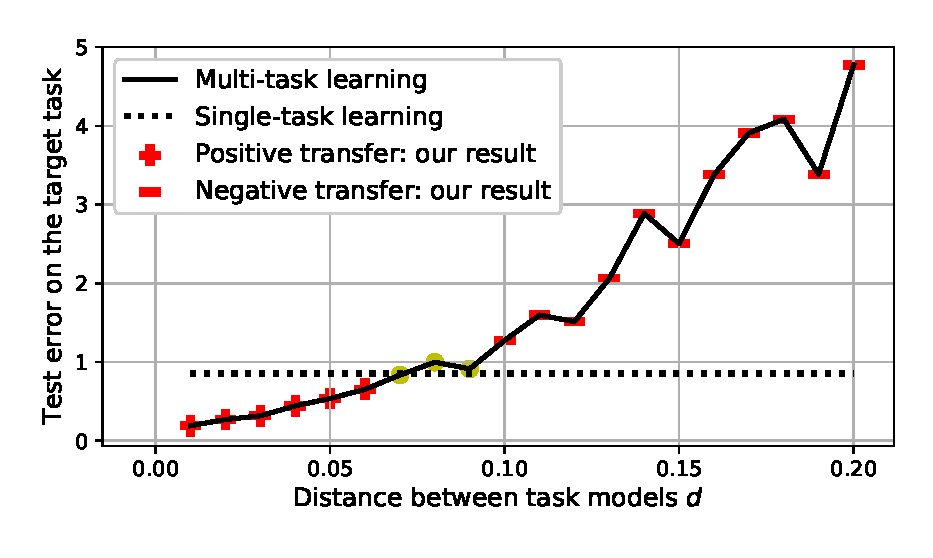
\includegraphics[width=0.98\textwidth]{figures/model_shift_phase_transition.eps}
		\caption{Task model similarity}
	\end{subfigure}\hfill
	\begin{subfigure}[b]{0.31\textwidth}
		\centering
		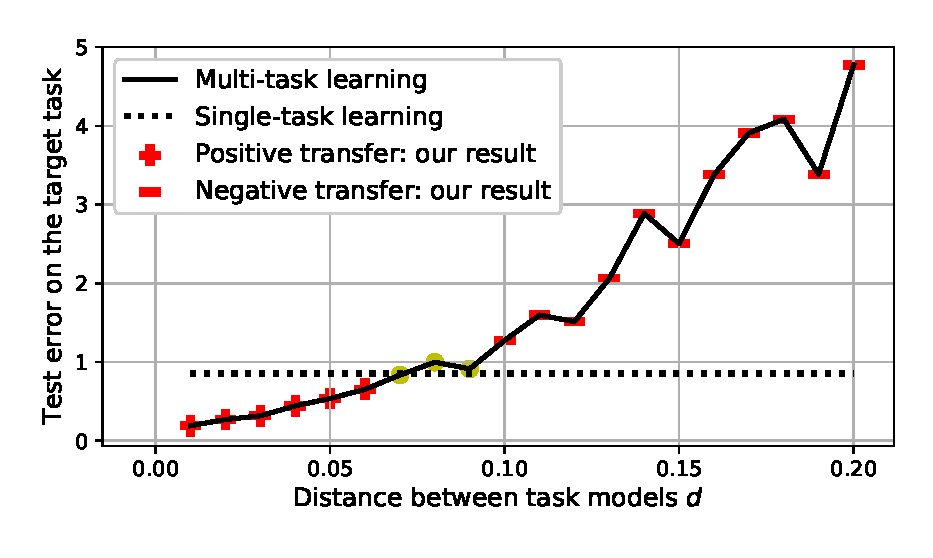
\includegraphics[width=0.98\textwidth]{figures/model_shift_phase_transition.eps}
		\caption{Source task noise level}
	\end{subfigure}\hfill
	\begin{subfigure}[b]{0.31\textwidth}
		\centering
		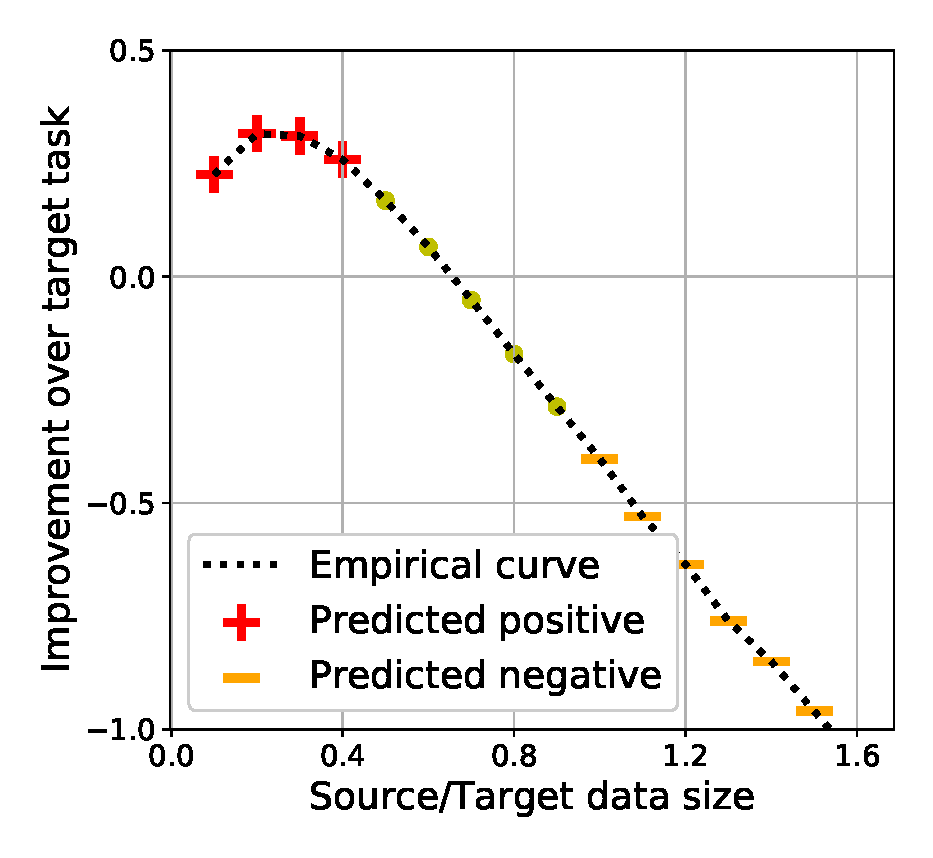
\includegraphics[width=0.98\textwidth]{figures/datapoints_phase_transition.eps}
		\caption{\# Source task datapoints}
	\end{subfigure}
	\caption{Comparing the test error of multi-task learning to single-task learning: we observe transitions from positive to negative transfer as a parameter of: (a) Task model similarities (Proposition \ref{prop_dist_transition}); (b) Source task noise level (Proposition \ref{prop_var_transition}); (c) Source task datapoints (Proposition \ref{prop_data_size}).}
	\label{fig_model_shift_phasetrans}
\end{figure}


Consider a more general setting where the noise level $\sigma_1$ of task $1$ differs from the noise level $\sigma_2$ of task $2$.
We derive a sharp transition similar to Proposition \ref{prop_dist_transition}.

\begin{proposition}\label{prop_var_transition}
	In the setting of Example \ref{ex_basic} with $d$ being fixed but $\sigma_1$ varies, assume that $c_1 > 100$ is a fixed constant and $d^2 < \frac {2\sigma^2} {3p} \frac{(c_1 + c_2 -1)^2}{c_1 (c_1 + c_2)(c_2 - 1)}$. Then we derive the following transition as a parameter of $\sigma_1$:
	\begin{itemize}
		\item If $\sigma_1^2 \le p d^2 \cdot c_1 +\left[1+ \frac23\frac{(c_1 + c_2 - 1)^2}{(c_1 + c_2) (c_2 - 1)}\right]\cdot\sigma_2^2$, then whp $\te(\hat{\beta}_t^{\MTL}) < \te(\hat{\beta}_t^{\STL})$.
		\item If $\sigma_1^2 > p d^2 \cdot c_1 +\left[1+ \frac32\frac{(c_1 + c_2 - 1)^2}{(c_1 + c_2) (c_2 - 1)}\right] \cdot \sigma_2^2$, then whp $\te(\hat{\beta}_t^{\MTL}) > \te(\hat{\beta}_t^{\STL})$.
	\end{itemize}
\end{proposition}

\textbf{Implications.} \todo{add connection to tasksonomy}

\subsection{Data Size and Efficiency}

In classical Rademacher or VC based theory of multi-task learning, adding more labeled data improves the generalization performance of a model.
On the other hand, we have observed that adding more labeled data does not always improve performance in multi-task learning.
Using Example \ref{ex_basic}, we analyze the effect of varying the source task data size.

\begin{proposition}\label{prop_data_size}
	In the setting of Example \ref{ex_basic}, assume that $c_2  \ge 3$ is fixed and $c_1 > a$ for some fixed integer $a$.	We have the following conditions to determine whether $\te(\hat{\beta}_t^{\MTL})$ is lower than $\te(\hat{\beta}_t^{\STL})$:
	\begin{itemize}
\item If $d^2 \le (1 + a^{-1/2})^{-4}\frac{\sigma^2}{p(c_2-1)}$, then whp $\te(\hat{\beta}_t^{\MTL}) < \te(\hat{\beta}_t^{\STL})$. 
		 
\item If $d^2 > (1 - a^{-1/2})^{-4}\frac{\sigma^2}{p (c_2 - 1)}$, then we have the following transition depending on $c_1$:
		\begin{itemize}
			\item If $c_1 < \frac{(c_2-2)\sigma^2}{(1+a^{-1/2})^4(c_2 - 1) pd^2 - \sigma^2}$, then whp $\te(\hat{\beta}_t^{\MTL}) < \te(\hat{\beta}_t^{\STL})$.
			\item If $c_1 > \frac{(c_2-2) \sigma^2}{(1-a^{-1/2})^4(1-(a+c_2-2)^{-2})(c_2 - 1) pd^2 - \sigma^2}$, then whp $\te(\hat{\beta}_t^{\MTL}) > \te(\hat{\beta}_t^{\STL})$.
		\end{itemize}
	\end{itemize}
\end{proposition}

The proof of Proposition \ref{prop_data_size} is similar to Proposition \ref{prop_dist_transition}.
We compare the model shift bias and the amount of reduced variance of $\hat{\beta}_t^{\MTL}$.
An intuitive interpretation of Proposition \ref{prop_data_size} is that:
i) If the two task models are sufficiently similar (as specified under the first bullet), adding the source task always provides positive transfer;
ii) Otherwise, as we increase the number of source task data points, the transfer is positive initially, but transitions to negative eventually.
We leave the proof of Proposition \ref{prop_data_size} to Appendix \ref{app_proof_data}.

\textbf{Implications.} We use our tools to explain a key result of taskonomy \cite{ZSSGM18}, which shows that by learning from multiple related tasks, one can reduce the amount of labeled data from each task.
This is formalized by a metric called the data efficiency ratio as follows.
Given several tasks, let $\alpha^{\star}$ be the largest factors such that the total number of labeled datapoints needed for solving all the tasks can be reduced by an $\alpha^{\star}$ factor (compared to training independently) while keeping the performance nearly the same.
More precisely, suppose we have $n_i$ datapoints for each task, for $i= 1, 2$.
If we only use $\alpha n_i$ datapoints from every task to train the multi-task learning estimator $\hat{\beta}(\alpha)$, then $\alpha \in (0, 1)$ will be the smallest number such that
\[ \alpha^{\star} \define\argmin_{\alpha\in(0, 1)} ~~ \te_1(\hat{\beta}(\alpha)) + \te_2(\hat{\beta}(\alpha))\le \te_1(\hat{\beta}_t^{\STL}) + \te_2(\hat{\beta}_t^{\STL}). \]
We quantify the data efficiency ratio of $\hat{\beta}_t^{\MTL}$ for Example \ref{ex_basic} as follows.

\begin{proposition}\label{prop_data_efficiency}
	In the setting of Example \ref{ex_basic}, assume that $c_1 = c_2 = c \ge 200$ and $d^2 < {8\sigma^2} /{(3p c)}$.
	Then the data efficiency ratio is at most $\frac{1}{2c} + \frac{\sigma^2}{2\sigma^2 - 3p d^2 c / 4}$.
\end{proposition}
Note that we have stated the result assuming that $c_1 = c_2$.
Similar results can also be obtained when they are different.
We omit the details.
The proof of Proposition \ref{prop_data_efficiency} can be found in Appendix \ref{app_proof_data}.




\subsection{Covariate Shift}

So far we have considered settings where $\Sigma_1 = \Sigma_2$.
This setting is relevant for multi-class image classification settings, where different tasks share the same input features.
In general, the covariance matrices of the two tasks may be different, e.g. in text classification.
In this part, we use our tools to provide a case study on the effect of applying multi-task learning for two tasks when $\Sigma_1 \neq \Sigma_2$.

For this setting, covariate shift is captured by the matrix $M = \Sigma_1^{1/2} \Sigma_2^{-1/2}$.
We ask: is it better to have $M$ as being close to identity, or should $M$ involve varying levels of singular values?
Understanding this question has implications for applying normalization methods in multi-task learning \cite{LV19,CBLR18,YKGLHF20}.
Our result shows that if $n_1$ is much larger than $n_2$, then the optimal $M$ matrix is equal to identity, under certain assumptions on its range of singular values (to be formulated in Proposition \ref{prop_covariate}).
On the other hand, if $n_1$ is comparable or even smaller than $n_2$, we show an example where having ``complementary'' covariance matrices is better performing than having the same covariance matrices.

\begin{example}\label{ex_cov_family}
	To compare different choices of $M$ on the performance of $\hat{\beta}_t^{\MTL}$, we assume an upper bound on the scale of $M$.
	Consider the following family of matrices
	\begin{align*}
		\cS_{\mu}\define\bigset{M \mid \det\bigbrace{ M^\top M} \le \mu^p, \lambda(M) \in [\mu_{\min}, \mu_{\max}]},
	\end{align*}
	where $\mu, \mu_{\min}, \mu_{\max}$ are fixed values that do not grow with $p$.
	For the task models, we assume that $\beta_2$ has i.i.d. entries with mean zero and variance $\kappa^2$ and $\beta_1 - \beta_2$ has i.i.d. entries with mean $0$ and variance $d^2$.
	The following proposition shows that when $n_1$ is large enough compared to $n_2$, $\te(\hat{\beta}^{\MTL})$ is minimized approximately within the family of $\cS_{\mu}$ when $M = \mu\id$.
\end{example}

\begin{proposition}\label{prop_covariate}
	In the setting of Example \ref{ex_basic}, assume that $c_1 > 3$ and $c_2>3$,
and $\|\Sigma_1\|\le C_1$ for some constant $C_1>0$. As a parameter of $M \in \cS_{\mu}$, we have that $(\te(\hat{\beta}_t^{\MTL}))(M)$ as a function of $M$ satisfies that 
\be\label{formular_covariate0} (\te(\hat{\beta}_t^{\MTL}))(\mu \id) \le \left[1+ C\left(c_2c_1^{-1} + c_1^{-1/2}\right)\right]\cdot\min_{M\in \cal S_{\mu}}(\te(\hat{\beta}_t^{\MTL}))(M) ,\ee
where the constant $C>0$ depends only on $\mu_{\max}$, $\mu_{\min}$ and $C_1$, but otherwise does not depend on $c_1$ and $c_2$. 
	%is minimized when $M = \mu\id$.
\end{proposition}

Proposition \ref{prop_covariate} shows that when $n_1\gg n_2$, $te(\hat{\beta}_t^{\MTL})$ is minimized when $\Sigma_1$ and $\Sigma_2$ are proportional to each other.
In other words, there is no covariate shift between the source task data and target task data.
This provides evidence that covariate shift is unfavorable when there are many source task datapoints,
To complement the result, we show an example when the statement is not true if $n_1 \le n_2$.

\begin{example}\label{ex_covariate}
	Within the setting of Example \ref{ex_cov_family}, we compare two cases: (i) when $M = \id$; (ii) when $M$ has $p/2$ singular values that are equal to $\lambda$ and $p/2$ singular values that are equal to $1 / \lambda$.
	For simplicity, we assume that $d = 0$.
	Hence the two tasks have the same model parameters.
%	now consider another case when $\Sigma_1$ and $\Sigma_2$ have complementary eigenspaces. Suppose $\Sigma_1$ and $\Sigma_2$ have the eigendecomposition
%$$\Sigma_1^{1/2} = 1+ U\Lambda U^\top, \quad \Sigma_2^{1/2} = 1+ V\Lambda V,$$
%where
%$$\Lambda = \diag(\wt\lambda_1,\cdots, \wt\lambda_{p/2}), \quad U= (u_1,\cdots, u_{p/2}), \quad V= (v_1,\cdots, v_{p/2}).$$
%If $V=U_\perp$, i.e. the vectors $v_1,\cdots, v_{p/2}$ are perpendicular to the vectors $u_1,\cdots, u_{p/2}$, then
%$$M=\Sigma_1^{1/2} \Sigma_2^{-1/2}=(1+\Lambda)UU^\top + (1+\Lambda)^{-1}V V^\top .$$
%	As a concrete example we consider the case where $\wt \lambda_1=\cdots=\wt\lambda_{p/2}$ and we denote $\lambda:=1+\wt\lambda_1$. Thus for $M$, the first $p/2$ singular values are equal to $\lambda$ and the rest ones are equal to $\lambda^{-1}$.

	In Figure \ref{fig_te_complement}, we plot the test error of the target task for $n_2 = 4p$ and $n_1$ ranging from $p$ to $20p$.
	Second, we observe the following two phases as we increase $n_1 / p$.
	\begin{itemize}
		\item When $n_1 \le n_2$, having complementary covariance matrices leads to lower test error compared to the case when $\Sigma_1 = \Sigma_2$.
		\item When $n_1 > n_2$, having complementary covariance matrices leads to higher test error compared to the case when $\Sigma_1 = \Sigma_2$.
	\end{itemize}
\end{example}

A theoretical justification of Example \ref{ex_covariate} can be found in Appendix \ref{app_covariate}.

\begin{figure}
	\begin{minipage}{0.48\textwidth}
		\centering
		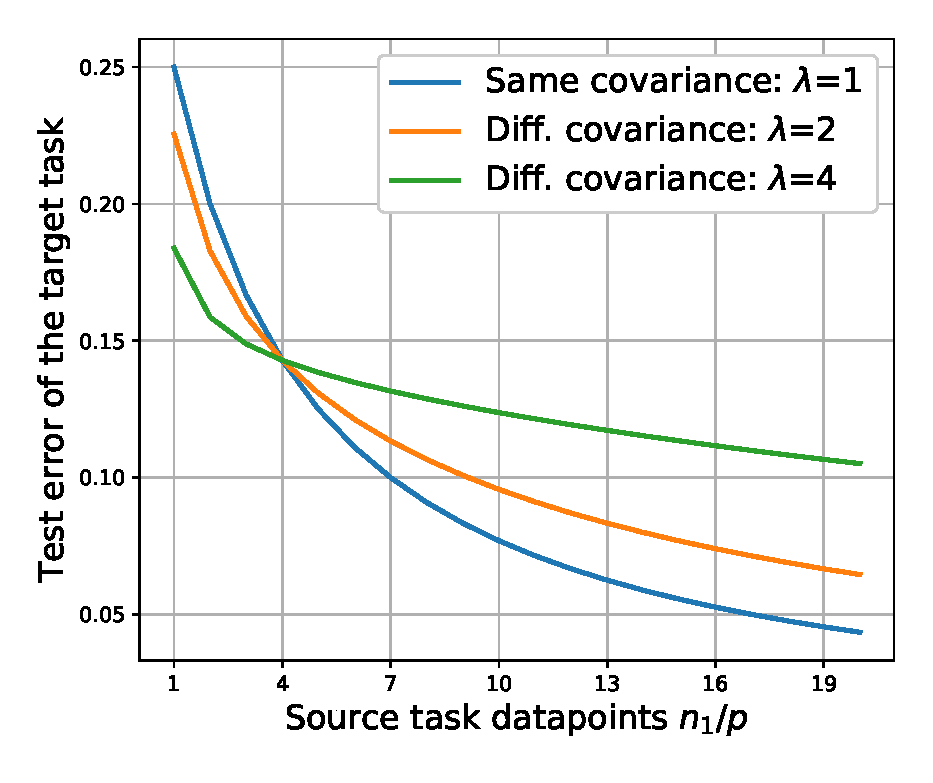
\includegraphics[width=0.9\textwidth]{figures/complementary.eps}
		\caption{When $\Sigma_1$ and $\Sigma_2$ are complementary. The number of target task data points is $n_2 = 4p$.}
		\label{fig_te_complement}
	\end{minipage}
\end{figure}

\textbf{Implications.}

